Experience shows that no single machine learning scheme is appropriate
to all data mining problems. The universal learner is an idealistic
fantasy. As we have emphasized throughout this book, real datasets
vary, and to obtain accurate models the bias of the learning algorithm
must match the structure of the domain. Data mining is an experimental
science.

The Weka workbench is a collection of state-of-the-art machine
learning algorithms and data preprocessing tools. It includes
virtually all the algorithms described in this book. It is designed so
that you can quickly try out existing methods on new datasets in
flexible ways. It provides extensive support for the whole process of
experimental data mining, including preparing the input data,
evaluating learning schemes statistically, and visualizing the input
data and the result of learning. As well as a wide variety of learning
algorithms, it includes a wide range of preprocessing tools. This
diverse and comprehensive toolkit is accessed through a common
interface so that its users can compare different methods and identify
those that are most appropriate for the problem at hand.

Weka was developed at the University of Waikato in New Zealand; the
name stands for \textit{Waikato Environment for Knowledge
Analysis}. Outside the university the weka, pronounced to rhyme with
Mecca, is a flightless bird with an inquisitive nature found only on
the islands of New Zealand. The system is written in Java and
distributed under the terms of the GNU General Public License. It runs
on almost any platform and has been tested under Linux, Windows, and
Macintosh operating systems—and even on a personal digital
assistant. It provides a uniform interface to many different learning
algorithms, along with methods for pre- and postprocessing and for
evaluating the result of learning schemes on any given dataset.

\section{What's in Weka?}

Weka provides implementations of learning algorithms that you can
easily apply to your dataset. It also includes a variety of tools for
transforming datasets, such as the algorithms for discretization
described in Chapter 8. You can preprocess a dataset, feed it into a
learning scheme, and analyze the resulting classifier and its
performance—--all without writing any program code at all.

The workbench includes methods for the main data mining problems:
regression, classification, clustering, association rule mining, and
attribute selection. Getting to know the data is an integral part of
the work, and many data visualization facilities and data
preprocessing tools are provided. All algorithms take their input in
the form of a single relational table in the ARFF format described in
Section 2.4, which can be read from a file or generated by a database
query.

One way of using Weka is to apply a learning method to a dataset and
analyze its output to learn more about the data. Another is to use
learned models to generate predictions on new instances. A third is to
apply several different learners and compare their performance in
order to choose one for prediction. In the interactive Weka interface
you select the learning method you want from a menu. Many methods have
tunable parameters, which you access through a property sheet or
\textit{object editor}. A common evaluation module is used to measure the
performance of all classifiers.
 
Implementations of actual learning schemes are the most valuable
resource that Weka provides. But tools for preprocessing the data,
called \textit{filters}, come a close second. Like classifiers, you select
filters from a menu and tailor them to your requirements. We will show
how different filters can be used, list the filtering algorithms, and
describe their parameters. Weka also includes implementations of
algorithms for learning association rules, clustering data for which
no class value is specified, and selecting relevant attributes in the
data, which we describe briefly.

\section{How do you use it?}

The easiest way to use Weka is through a graphical user interface
called the \textit{Explorer}. This gives access to all of its
facilities using menu selection and form filling. For example, you can
quickly read in a dataset from an ARFF file (or spreadsheet) and build
a decision tree from it. But learning decision trees is just the
beginning: there are many other algorithms to explore. The Explorer
interface helps you do just that. It guides you by presenting choices
as menus, by forcing you to work in an appropriate order by graying
out options until they are applicable, and by presenting options as
forms to be filled out. Helpful \textit{tool tips} pop up as the mouse
passes over items on the screen to explain what they do. Sensible
default values ensure that you can get results with a minimum of
effort—--but you will have to think about what you are doing to
understand what the results mean.

There are three other graphical user interfaces to
Weka. The \textit{Knowledge Flow} interface allows you to design
configurations for streamed data processing. A fundamental
disadvantage of the Explorer is that it holds everything in main
memory—--when you open a dataset, it immediately loads it all in. That
means that it can only be applied to small to medium-sized
problems. However, Weka contains some incremental algorithms that can
be used to process very large datasets. The Knowledge Flow interface
lets you drag boxes representing learning algorithms and data sources
around the screen and join them together into the configuration you
want. It enables you to specify a data stream by connecting components
representing data sources, preprocessing tools, learning algorithms,
evaluation methods, and visualization modules. If the filters and
learning algorithms are capable of incremental learning, data will be
loaded and processed incrementally.

Weka’s third interface, the \textit{Experimenter}, is designed to help
you answer a basic practical question when applying classification and
regression techniques: which methods and parameter values work best
for the given problem? There is usually no way to answer this question
a priori, and one reason we developed the workbench was to provide an
environment that enables Weka users to compare a variety of learning
techniques. This can be done interactively using the
Explorer. However, the Experimenter allows you to automate the process
by making it easy to run classifiers and filters with different
parameter settings on a corpus of datasets, collect performance
statistics, and perform significance tests. Advanced users can employ
the Experimenter to distribute the computing load across multiple
machines using Java remote method invocation (RMI). In this way you
can set up large-scale statistical experiments and leave them to run.

The fourth interface, called the \textit{Workbench}, is a unified
graphical user interface that combines the other three (and any
plugins that the user has installed) into one application. The
Workbench is highly configurable, allowing the user to specify which
applications and plugins will appear, along with settings relating to
them.

Behind these interactive interfaces lies the basic functionality of
Weka. This can be accessed in raw form by entering textual commands,
which gives access to all features of the system. When you fire up
Weka you have to choose among four different user interfaces: the
Explorer, Knowledge Flow, Experimenter, and command-line
interfaces. We describe them in turn in the next chapters. Most people
choose the Explorer, at least initially.

\section{What else can you do?}

An important resource when working with Weka is the online
documentation, which has been automatically generated from the source
code and concisely reflects its structure. We will explain how to use
this documentation. We will also identify Weka’s major building
blocks, highlighting which parts contain supervised learning methods,
which contain tools for data preprocessing, and which contain methods
for other learning schemes. The online documentation gives the only
complete list of available algorithms because Weka is continually
growing and--—being generated automatically from the source code--—the
online documentation is always up to date. Moreover, it becomes
essential if you want to proceed to the next level and access the
library from your own Java programs or write and test learning schemes
of your own.

In most data mining applications, the machine learning component is
just a small part of a far larger software system. If you intend to
write a data mining application, you will want to access the programs
in Weka from inside your own code. By doing so, you can solve the
machine learning subproblem of your application with a minimum of
additional programming. We show how to do that by presenting an
example of a simple data mining application in Java. This will enable
you to become familiar with the basic data structures in Weka,
representing instances, classifiers, and filters.

If you intend to become an expert in machine learning algorithms (or,
indeed, if you already are one), you’ll probably want to implement
your own algorithms without having to address such mundane details as
reading the data from a file, implementing filtering algorithms, or
providing code to evaluate the results. If so, we have good news for
you: Weka already includes all this. To make full use of it, you must
become acquainted with the basic data structures. To help you reach
this point, we will describe these structures in more detail and
explain an illustrative implementation of a classifier.

\section{How do you get it?}

Weka is available from http://www.cs.waikato.ac.nz/ml/weka. You can
download either a platform-specific installer or an executable Java jar
file that you run in the usual way if Java is installed. We recommend
that you download and install it now, and follow through the examples
in the upcoming sections.

\section{The package management system}

The Weka software has evolved considerably since the third edition of
this book was published. Many new algorithms and features have been
added to the system, a number of which have been contributed by the
community. With so many algorithms on offer we felt that the software
could be considered overwhelming to the new user. To aleviate this, a
number of core algorithms and community contributions were removed and
placed into plugin \textit{packages}. A package management system was
added that allows the user to browse for, and selectively install,
packages of interest.

\begin{figure}[!th]
\centering
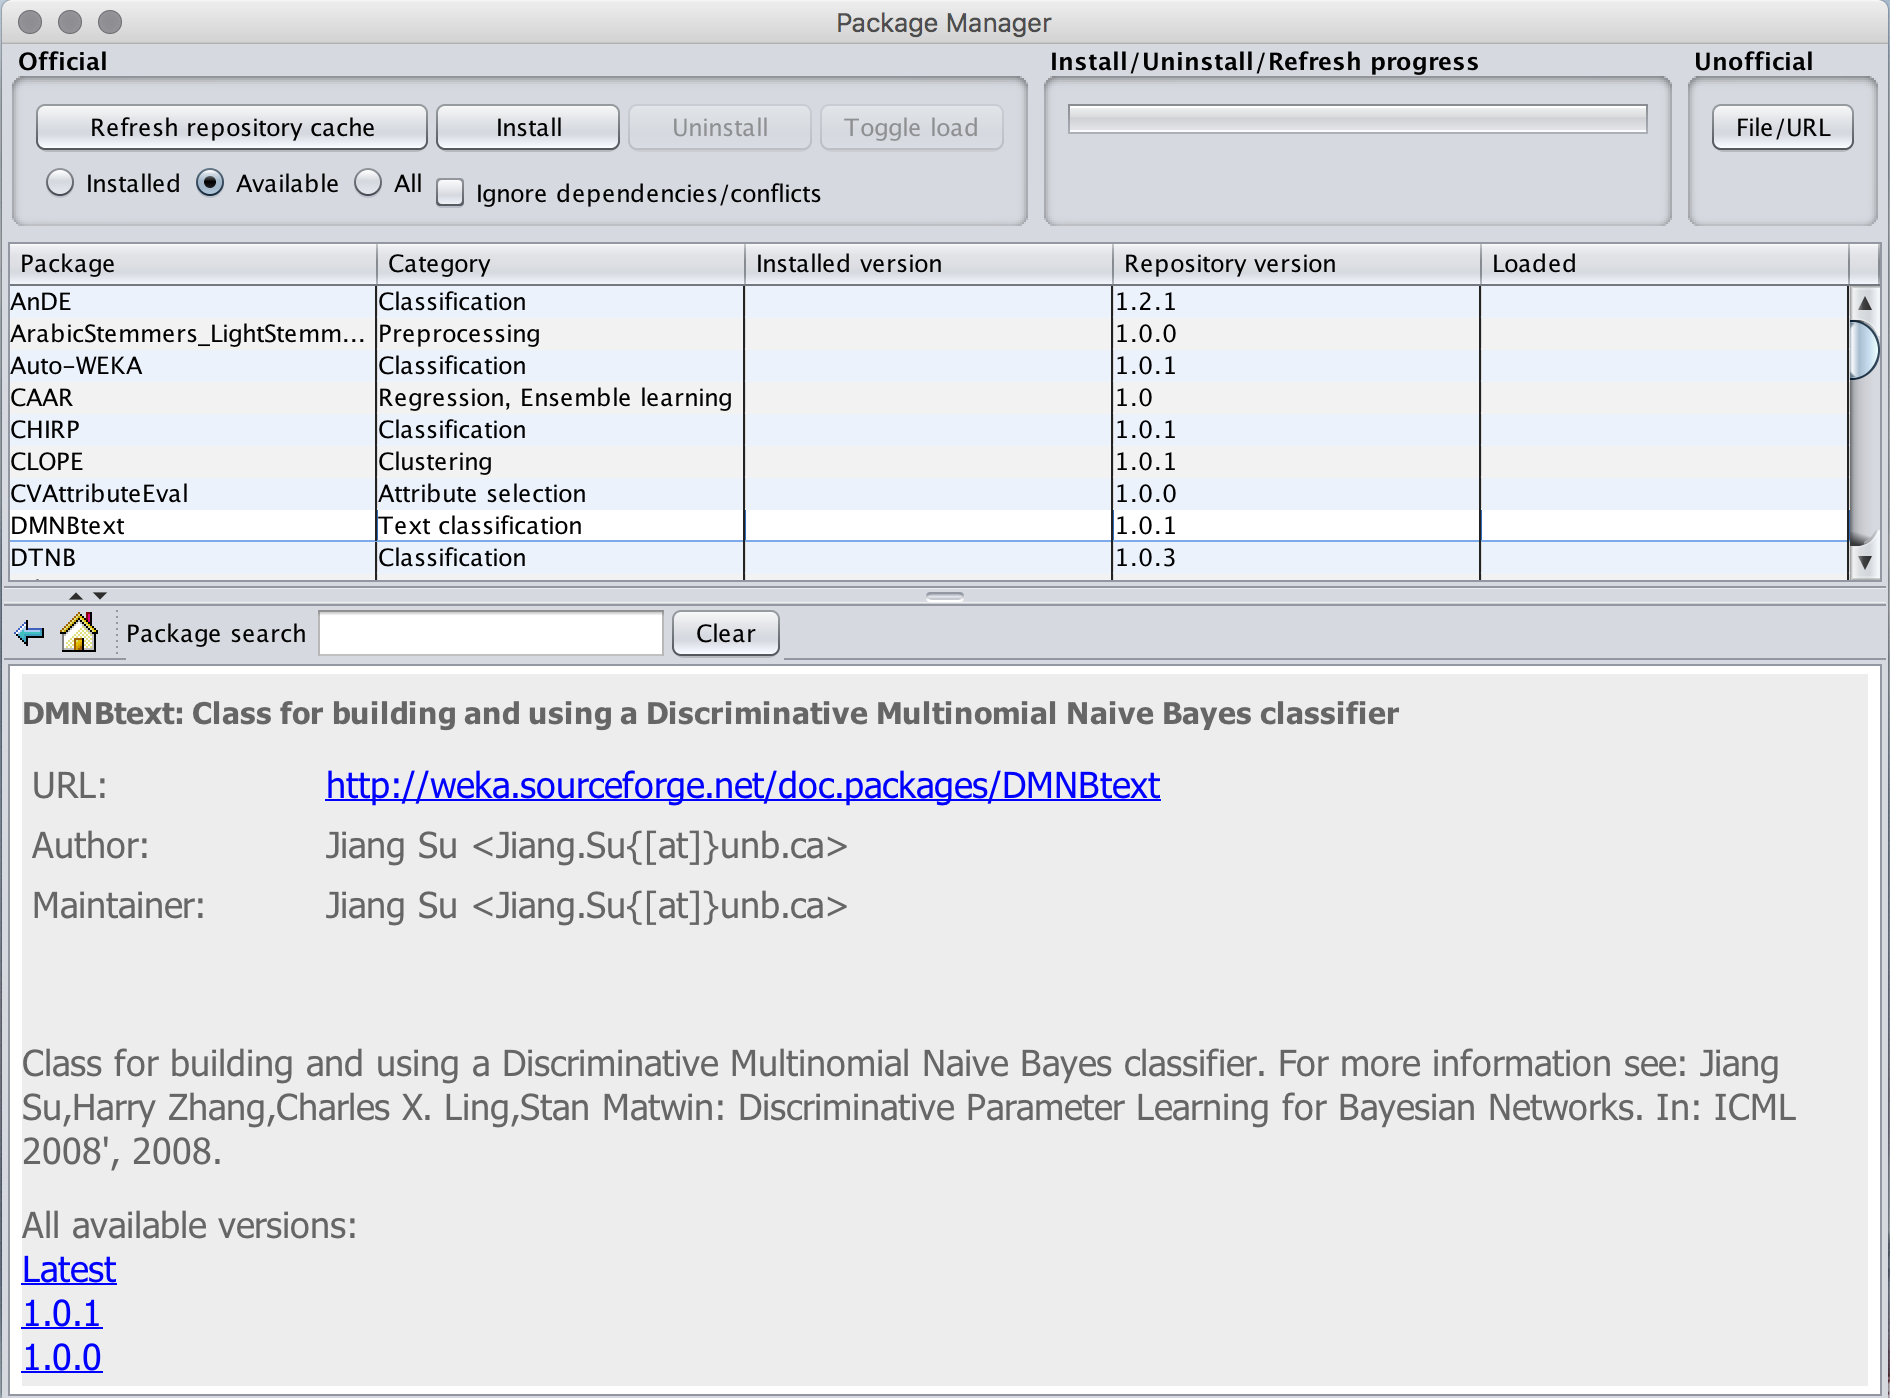
\includegraphics[width=0.9\textwidth]{images/P1.png}
\caption{The graphical package manager.}
\label{fig:package_manager}
\end{figure}

Another motivation for introducing the package management system was
to make the process of contributing to the Weka software easier, and
to ease the maintenance burden on the Weka development team. A
contributor of a plugin package is responsible for maintaining its
code and hosting the installable archive; while Weka simply tracks the
package metadata. The package system also opens the door to the use of
third-party libraries, something that we'd discouraged in the past in
order to keep a lightweight footprint for Weka.

\begin{figure}[!th]
\centering
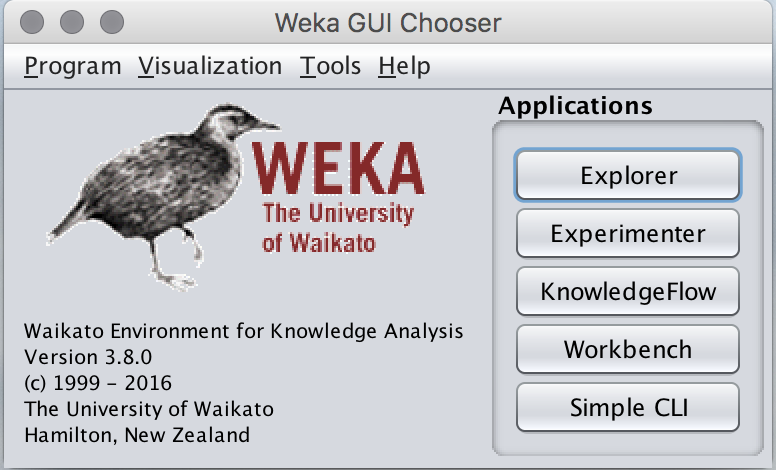
\includegraphics[width=0.6\textwidth]{images/B_2_3a.png}
\caption{The GUI Chooser.}
\label{fig:gui_chooser}
\end{figure}

Figure~\ref{fig:package_manager} shows the main window of the
graphical package manger, which can be accessed from the Tools menu in
the \textit{GUI Chooser} panel shown in
Figure~\ref{fig:gui_chooser}. The very first time the package manager
is accessed it will download information about the currently available
packages. This requires an internet connection, however, once the
package metadata has been downloaded it is possible to use the package
manager to browse package information while offline. Of course, an
internet connection is still required to be able to actually install a
package.

\begin{figure}[!th]
\centering
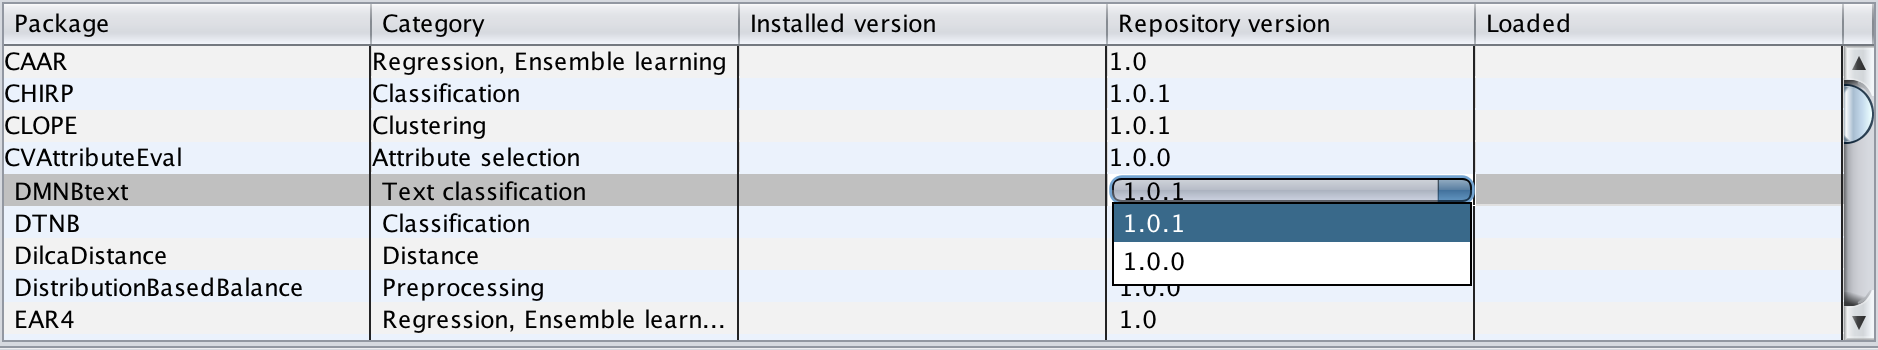
\includegraphics[width=0.9\textwidth]{images/P2.png}
\caption{Choosing a version of the \textit{DMNBtext} package to install.}
\label{fig:package_manager_2}
\end{figure}

The package manager presents a list of packages near the top of the
window and a panel at the bottom that displays information on the
currently selected package in the list. The user can choose to display
packages that are available (i.e. not yet installed), only packages
that are installed, or all packages. The list presents the name of
each package, the broad category that it belongs to, the version
currently installed (if any), the most recent version of the package
available that is compatible with the version of Weka being used, and
a field that, for installed packages, indicates whether the package
has been loaded successfully by Weka or not. Although not obvious at
first glance, it is possible to install older versions of a particular
package. The Repository version field in the list is actually a
drop-down box. Figure~\ref{fig:package_manager_2} shows selecting a
version of the \textit{DMNBtext} package to install. The list of
packages can be sorted, in ascending or descending order, by clicking
on either the package or category column header.

\begin{figure}[!th]
\centering
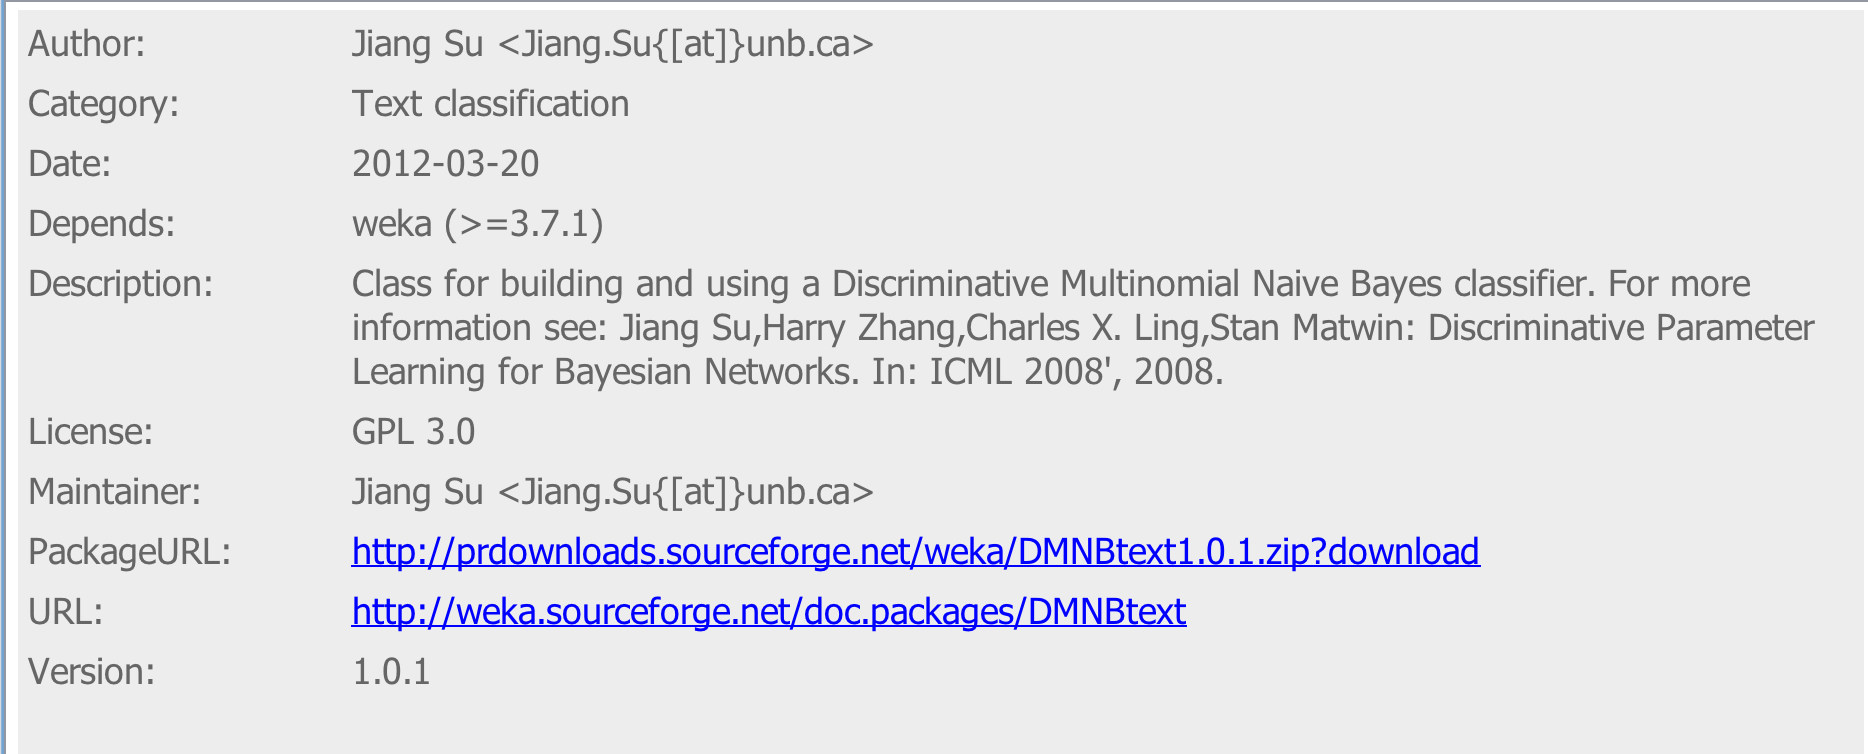
\includegraphics[width=0.9\textwidth]{images/P3.png}
\caption{Additional information for the \textit{DMNBtext} package.}
\label{fig:package_manager_3}
\end{figure}

\begin{figure}[!th]
\centering
\subfloat[Primary package.]{\label{subfig:pm_1}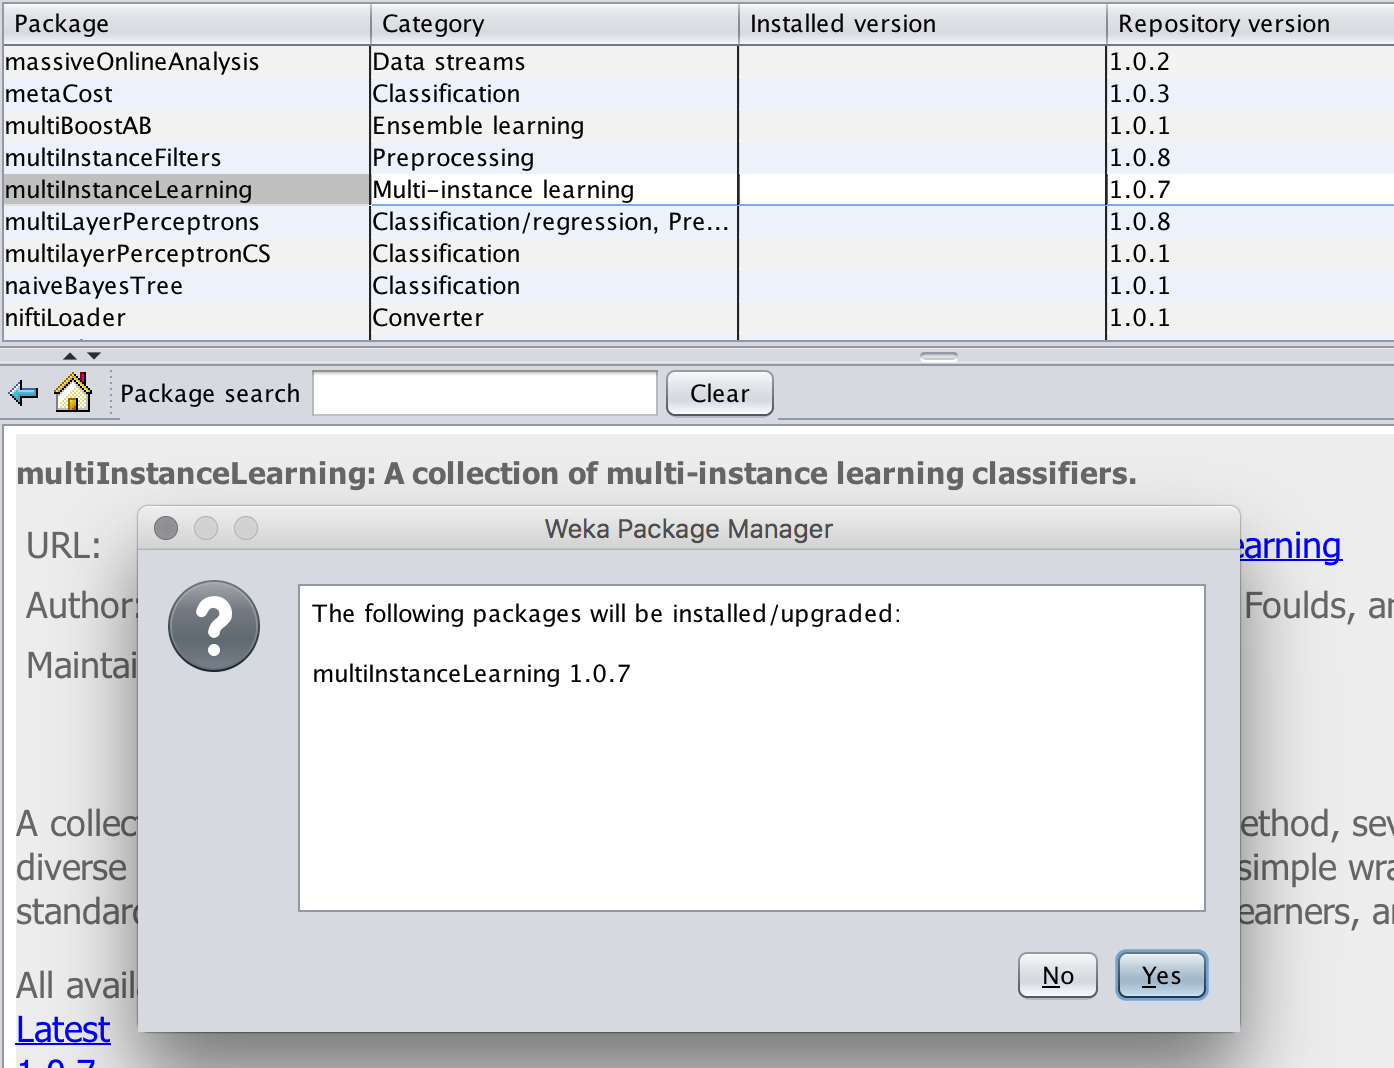
\includegraphics[width=0.45\textwidth]{images/P4a.png}}
\qquad
\subfloat[Dependency.]{\label{subfig:pm_2}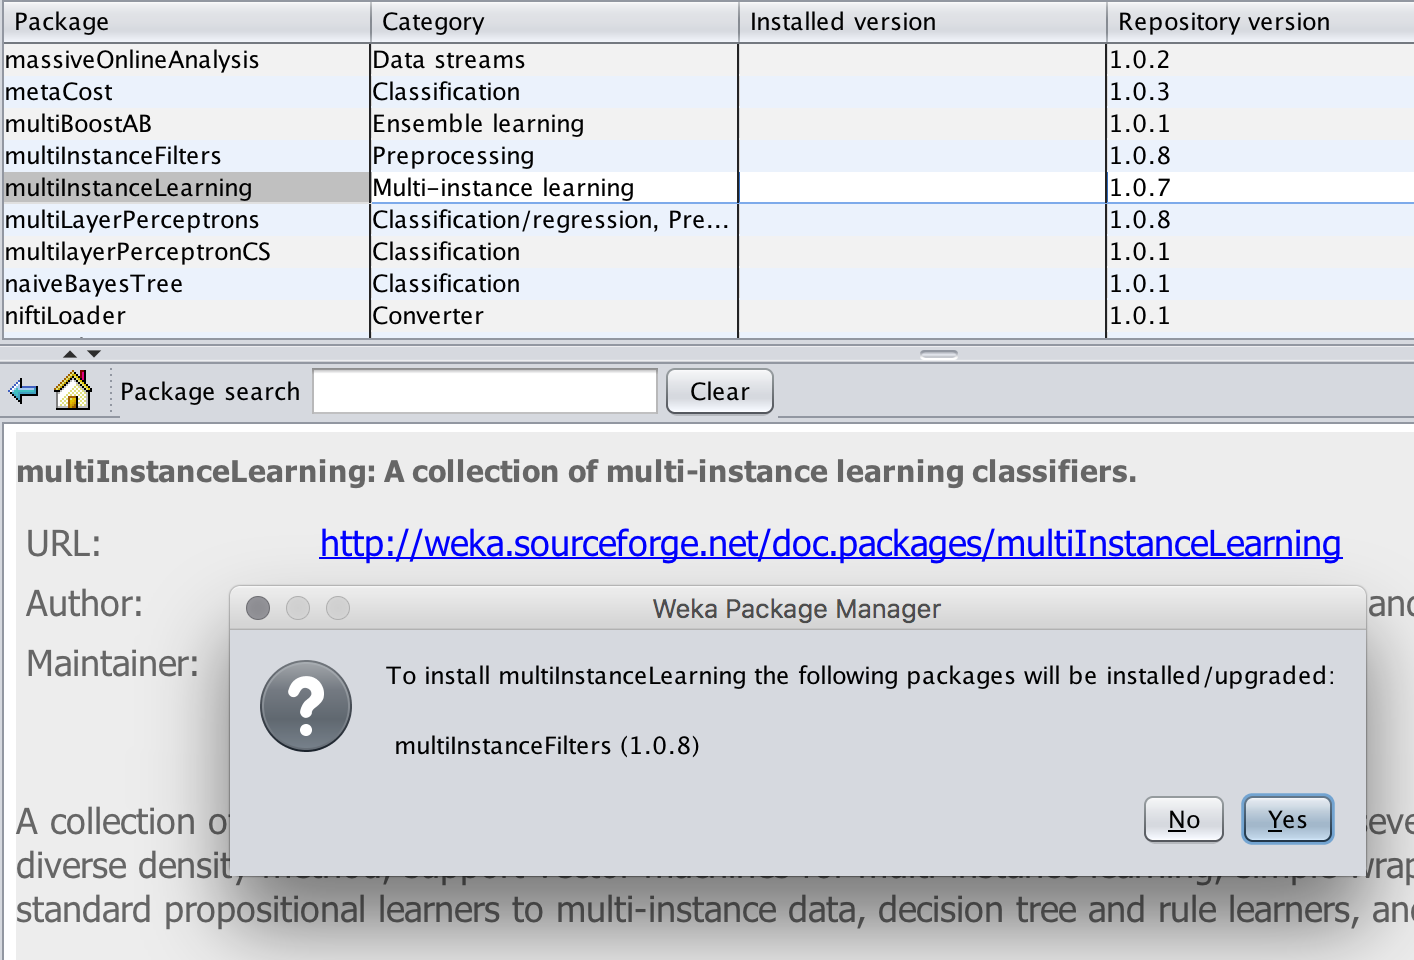
\includegraphics[width=0.45\textwidth]{images/P4b.png}}
\caption{\label{fig:package_manager_4}Installing a package with dependencies.}
\end{figure}

The information panel at the bottom of the window has clickable links
for each version of a given package. ``Latest'' always refers to the
latest version of the package, and is the same as the highest version
number available. Clicking one of these links displays further
information, such as the author of the package, its license, where the
installable archive is located, and its
dependencies. Figure~\ref{fig:package_manager_3} shows this
information for the \textit{DMNBtext} package. The information about
each package is also browsable at the web location where Weka's
package metadata is hosted. At the time of writing this can be found
at http://weka.sourceforge.net/packageMetaData/. All packages have at
least one dependency listed – the minium version of the core Weka
system that they can work with. Some packages list further
dependencies on other packages. For example,
the \textit{multiInstanceLearning} package depends on the
\textit{multiInstanceFilters} package. When installing \textit{multiInstanceLearning},
and assuming that \textit{multiInstanceFilters} is not already
installed, the system will inform the user the \textit{multiInstanceFilters} is
required and will be installed automatically. Figure~\ref{fig:package_manager_4} shows the
dialogs displayed by the package manager when installing
\textit{multiInstanceLearning}.

The package manager displays what are known as \textit{official} packages for
Weka. These are packages that have been submitted to the Weka team for
a cursory review and have had their metadata added to the official
central metadata repository. For one reason or another, an author of a
package might decide to make it available in an unofficial
capacity. These packages do not appear in the official list on the
web, or in the list displayed by the graphical package manager. If the
user knows the URL to an archive containing an unofficial package, it
can be installed by using the button in the upper right-hand corner of
the package manager window.

\begin{figure}[!th]
\centering
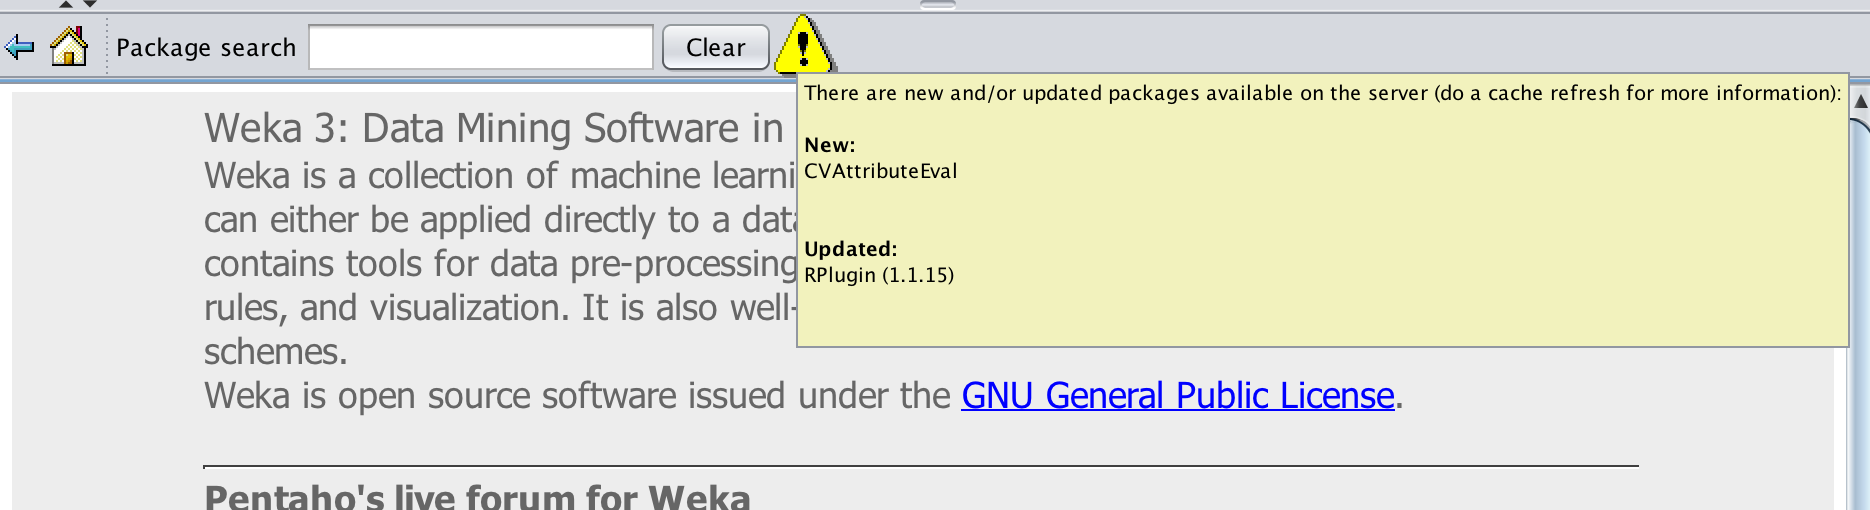
\includegraphics[width=0.9\textwidth]{images/P5.png}
\caption{New/updated packages available.}
\label{fig:package_manager_5}
\end{figure}

Whenever a new package, or new version of an existing one, becomes
available the package manager informs the user by displaying a large
yellow warning icon. Hovering over this icon displays a tool-tip popup
that lists the new packages and prompts the user to click
the \textit{Refresh repository cache} button. Clicking this button
downloads a fresh copy of all the package information to the user's
computer. Figure~\ref{fig:package_manager_5} shows what is displayed
in the situation where there is one new package avallable and one
upgrade to an existing package.

\begin{figure}[!th]
\centering
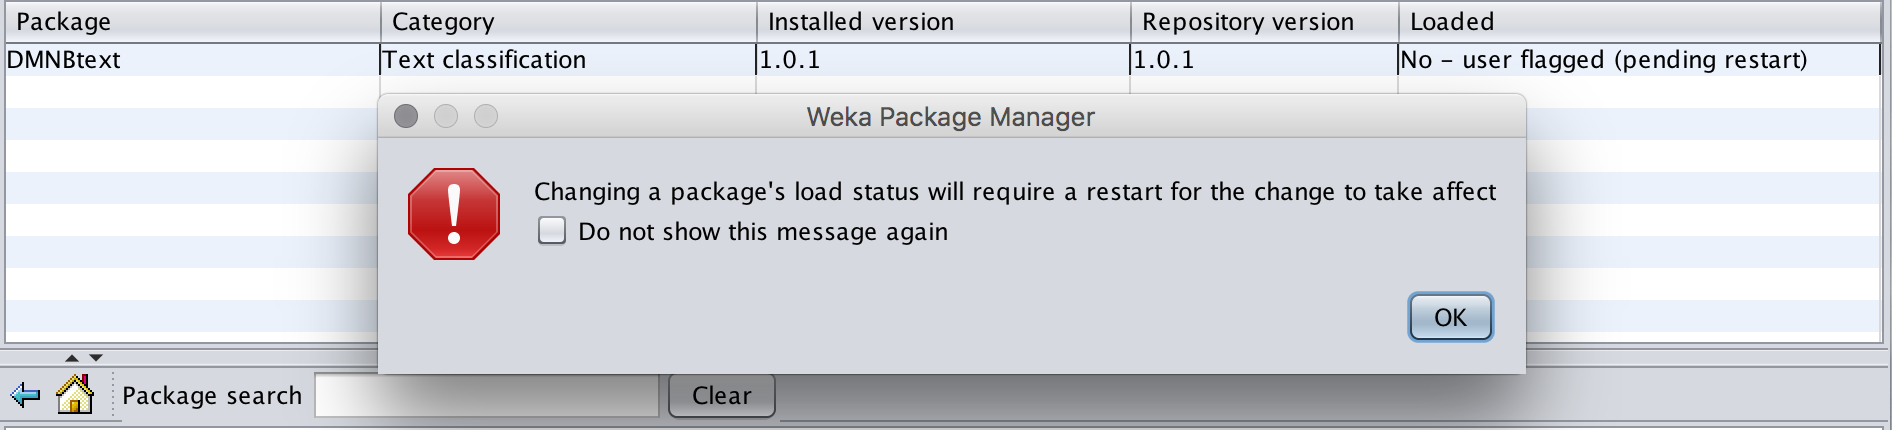
\includegraphics[width=0.9\textwidth]{images/P6.png}
\caption{Changing the load status of a package.}
\label{fig:package_manager_6}
\end{figure}

The \textit{Install} and \textit{Uninstall} buttons at the top of the
package manager's window do exactly as their names suggest. More than
one package can be installed or uninstalled in one go by by selecting
multiple entries in the list. By default, Weka attempts to load all
installed packages, and if a package can't be loaded for some reason a
message will be displayed in the \textit{Loaded} column of the
list. The user can opt to prevent a particular package from being
loaded by selecting it and then clicking the \textit{Toggle load}
button. This will mark the package as one that should not be loaded
the next time that Weka is started. This can be useful if an unstable
package is generating errors, conflicting with another package
(perhaps due to third party libraries), or otherwise preventing Weka
from operating properly. Figure P.6 shows what is displayed when a
package's load status is toggled.

